\chapter{Présentation du sujet}
\label{chap:presentation}
% Présentation générale %
%---------------------------------------------------------------------------%
\section{Présentation générale}
La détection d'objet est une technique de vision par ordinateur qui a pour but d'identifier un ou plusieurs objets dans une image et de les localiser en entourant chacun d'eux au moyen d'une boite englobante. De nos jours, cette technique est devenue incontournable au vu des nombreuses applications dans des domaines très variés, tels que la vidéo surveillance, les voitures autonomes, etc.

Bien que le sujet de la détection est étudié depuis longtemps, il n'existe toujours pas, à l'heure actuelle, de méthode permettant de réaliser une détection parfaite dans tous les cas. La recherche s'attelle donc à mettre au point des techniques permettant d'obtenir une détection la plus précise possible. Dans cette recherche de l'amélioration des performances pour les détecteurs, ces dernières années ont vu apparaître l'utilisation de méthodes de deep learning (à base de réseaux de neurones profonds) pour la vision. Ces méthodes ont permis de réaliser des progrès remarquables et d'atteindre une précision bien plus élevée qu'auparavant.

\begin{figure}[!ht]
  \centering
  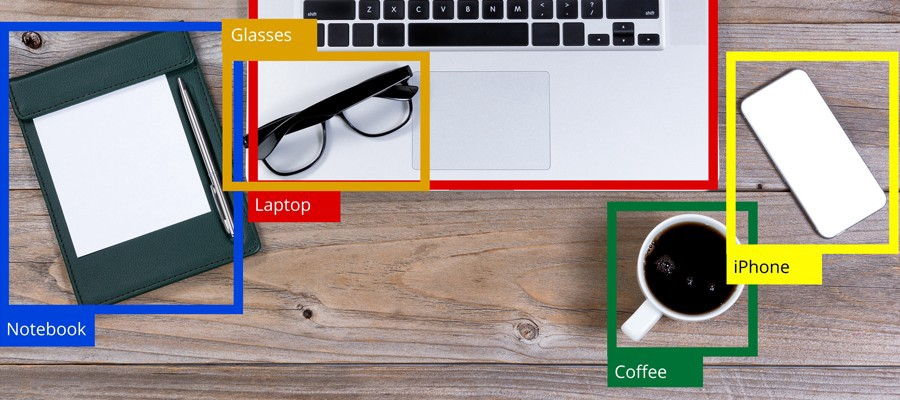
\includegraphics[width=8cm]{img/object-detection.jpeg}
  \caption{Exemple de détection d'objet}
  \label{fig:obj-det-example}
\end{figure}

Néanmoins, l'utilisation du deep learning introduit d'autres défis liés à la nature même des réseaux neuronaux. L'un des plus importants est celui de l'obtention et de l'annotation des données servant à entraîner un détecteur basé sur le deep learning. C'est dans cette problématique que réside le coeur de notre projet.


% Problématique %
%---------------------------------------------------------------------------%
\section{Problématique}
Les détecteurs basés sur des techniques de deep learning nécessitent d'être entraînés à reconnaître les objets voulus dans une image. Ceci est fait grâce à une phase d'entraînement, où on fournit au réseau de neurones une grande quantité d'images annotées à la main avec lesquelles il apprend à détecter les objets voulus. 

Un des plus grands problèmes dans l'utilisation de ces méthodes est l'obtention de ces images annotées. En effet, l'obtention de ces données annotées à la main est extrêmement coûteux puisqu'il faut, d'une part, obtenir ces images et d'autre part, marquer précisément chaque emplacement des objets grâce à des boîtes englobantes. De plus, le nombre d'images nécessaire est important ($\pm$ 330k images pour \cite{Lin_2014}, par exemple).

Sachant cela, il devient clair que le processus d'annotation manuel est coûteux en temps et en argent. Outre la nécessité de moyens importants, l'obtention de grande quantité de données à labéliser dans certains domaines d'application (en recherche médicale, par exemple) n'est tout simplement pas possible.

Avec ces constatations, nous pouvons formuler la problématique comme suit : \textbf{le besoin d'une très grande quantité de données supervisées manuellement constitue un verrou scientifique dans la conception de méthodes de détection d'objets dans des environnements où ces données ne sont pas accessibles. Il est donc nécessaire de créer des méthodes capables de travailler avec un volume de données réduit.}

% Objectif %
%---------------------------------------------------------------------------%
\section{Objectif}
Pour répondre à la problématique, la littérature scientifique travaille depuis peu à toute une série de méthodes qui diffèrent selon le contexte dans lequel elles peuvent être utilisées. Les résultats de ces solutions envisagées peuvent varier suivant leur niveau de précision et la réduction de quantité de données requises. L'objectif de notre projet est ainsi de faire un état de l'art puis une comparaison des solutions à cette problématique en répertoriant ces méthodes et leur contexte.